\documentclass[./main.tex]{subfiles}
\graphicspath{{\subfix{./Abbildungen/}}}
\begin{document}
{\centering\large\bfseries Spektroskopische Daten\par}

Multiplizit\"at eines Signals: $M = 2\cdot n\cdot I +1$\par

\begin{formulabox}[\textsuperscript{1}H: Chemische Verschiebung]
  \begin{center}
  \renewcommand{\arraystretch}{1.4}
    \begin{tabular}{c}
        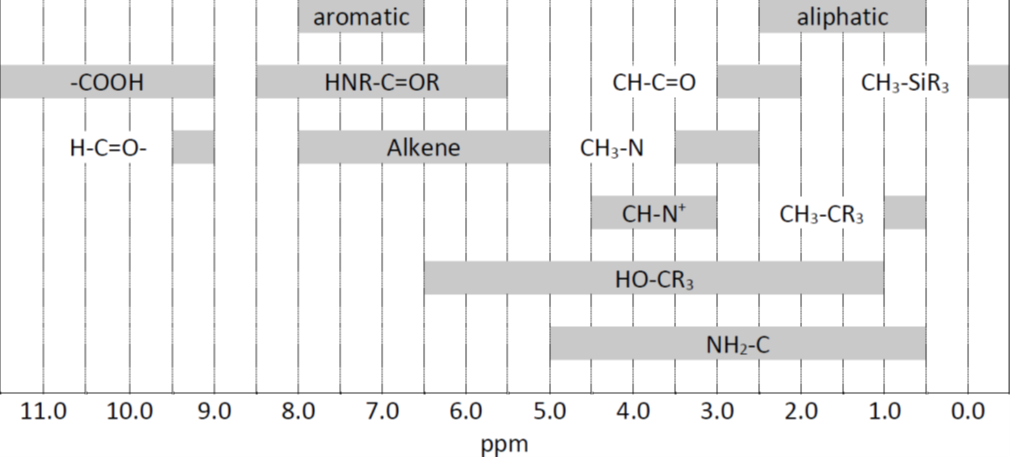
\includegraphics[width=\linewidth]{1H.png}
    \end{tabular}
  \end{center}
\end{formulabox}

\begin{formulabox}[\textsuperscript{13}C: Chemische Verschiebung]
  \begin{center}
  \renewcommand{\arraystretch}{1.4}
    \begin{tabular}{c}
        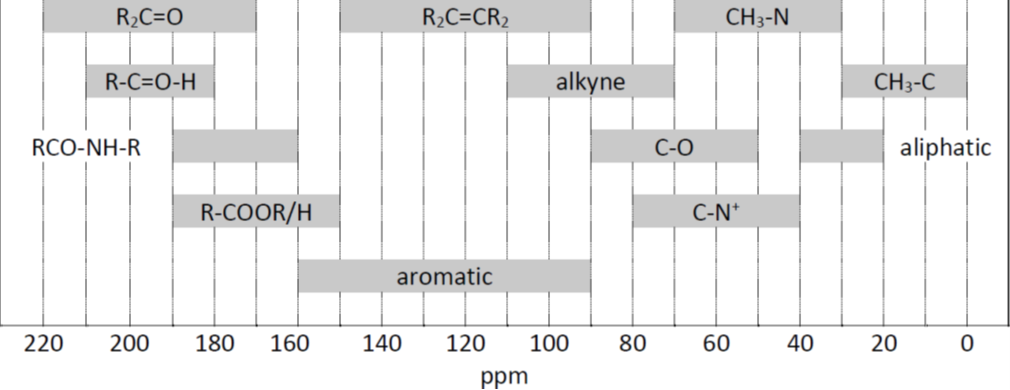
\includegraphics[width=\linewidth]{13C.png}
    \end{tabular}
  \end{center}
\end{formulabox}

\begin{formulabox}[\textsuperscript{1}H: Kopplungskonstanten ($J$ in Hz)]
  \begin{center}
  \renewcommand{\arraystretch}{1.2}
    \begin{tabular}{>{\raggedleft\arraybackslash}p{0.4\textwidth} p{0.02\textwidth}p{0.58\textwidth}}
        \ch{R2CH_aH_b} && 4 -- 20 \\
        \ch{R2CH_a-CR2H_b} && 2 -- 12 \\
        \ch{R2CH_a-CR2-CR2H_b} && freie Rotation: <0,1; fixed: 1 -- 8 \\
        \textit{cis}-\ch{RH_aC=CRH_b} && 7 -- 12 \\
        \textit{trans}-\ch{RH_aC=CRH_b} && 12 -- 18 \\
        \ch{R2C=CH_aH_b} && 0,5 -- 3 \\
        \ch{RH_aC=CR-CR2H_b} && 0,5 -- 2,5 \\
    \end{tabular}
  \end{center}
\end{formulabox}

\newpage
\end{document}
